%!TEX root = ../dissertation.tex
%\begin{savequote}[75mm]
%\qauthor{Quoteauthor Lastname}
%\end{savequote}

%% Set up problem
\begin{figure*}[t]
\begin{center}
{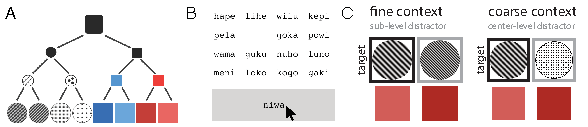
\includegraphics[scale=1.6]{./figures/Sec2-design.pdf}}
{\caption{{\emph{Domain for context-sensitivity.} (A) Targets are related to one another in a conceptual taxonomy. (B) Speakers choose between labels, where the label ``niwa'' has been selected. (C) Examples of \emph{fine} and \emph{coarse} contexts. In the \emph{fine} context, the target (marked in black) must be disambiguated from a distractor (marked in grey) at the same subordinate-level branch of the taxonomy.  In the \emph{coarse} context, the closest distractor belongs to a different branch of the center-level of the taxonomy (i.e. a spotted circle) such that disambiguation at the sub-ordinate level is not required. \label{fig:context_design}}}}
\end{center}
\end{figure*}

In the previous two sections, we examined a mechanism for rapid, partner-specific learning that allows agents to form stable but arbitrary \emph{ad hoc} conventions with partners and gradually generalize them to their entire community. 
The final phenomenon we consider is the way that \emph{ad hoc} conventions are shaped by the communicative context in which they form.
This phenomenon is most immediately motivated by recent behavioral results finding that more informative words in the local context are significantly more likely to become conventionalized \cite{hawkins2020characterizing}.

\todo[]{By 'communicative context' do you mean the linguistic context: e.g., referring expressions are more likely to remain than modifiers which is, I'd say, about the function of constructions; Or do you mean the non-linguistic context: e.g., when we need to distinguish narrow categories, we use more narrow terms? Or do you just mean that conventions are not predictable: i.e., a different group could converge on a different solution?}

%related: more important or more (likely to be) frequent?   %PREDICTABLE words tend to get reduced

\todo[]{need to say more (or less) about Optimal Semantic Expressivity (blogpost?); if the idea is that languages are as expressive and as efficient as possible, it's an old functionalist idea, but it's not entirely clear what you're alluding to here}
However, our broader theoretical aim is to suggest that \emph{diachronic} patterns in the long-term evolution of a community's lexical conventions, as highlighted by the Optimal Semantic Expressivity (OSE) hypothesis \cite{frankblogpost}, may be explained as a result of the \emph{synchronic} processes at play when individual dyads coordinate on  \emph{ad hoc} meanings.

\todo[]{incorporate footnote 1 into text somewhere or allude to footnote 1 again around here?  We focus here on reduction in referring expressions found in cases such as \textit{automobile > car; television > TV; the Jan 6th insurrection > Jan 6th}. We recognize that languages do not march inexorably toward efficiency. In particular, emphasis and politeness considerations regularly lead to lengthening of expressions. While saying someone \textit{died} may be efficient, longer formulations are more polite \textit{passed away}, \textit{deceased}. Negation in spoken French provides a standard example of initial lengthening for the purpose of emphasis: \textit{ne > ne pas}. If longer expressions no longer serve their original purpose, over time, they tend to be reduced   {ne pas > pas}.   }

Briefly, when there is already a strong existing convention that is expected to be shared across the community, our model predicts that speakers will use it. 
New \emph{ad hoc} conventions arise precisely to fill \emph{gaps} in existing population-level conventions, to handle new situations where existing conventions are not sufficient to accurately and efficiently make the distinctions that are required in the current context. 
A corollary of this prediction\footnote{This follows by induction from the hierarchical generalization mechanisms evaluated for $\textbf{P2}$, which provide the pathway by which \emph{ad hoc} conventions become adopted by a larger community over longer time scales. Many \emph{ad hoc} conventions never generalize to the full language community simply because the contexts where they are needed are rare. They must be re-negotiated with subsequent partners on an \emph{ad hoc} basis.} is that \emph{ad hoc} conventions may only shift to expectations at the population level (and ultimately to population-level convergence) when those distinctions are consistently relevant across interactions with different partners.
%Conversely, if the gap a convention was introduced to fill is rare or usually irrelevant, it may drop out of the lexicon; it is easier to re-negotiate \emph{ad hoc} conventions in each setting
For example, while most English speakers have the general term  ``tree'' in their lexicon, along with a handful of subordinate-level words like ``maple'' or ``fir,'' we typically do not have conventionalized labels exclusively referring to each individual tree in our yards -- we are rarely required to refer to individual trees.
Meanwhile, we \emph{do} often have shared conventions (i.e. proper nouns) for individual people and places that a community regularly encounters and needs to distinguish among.
Indeed, this logic may explain why a handful of particularly notable trees do have conventionalized names, such as the Fortingall Yew, the Cedars of God, and General Sherman, the giant sequoia.
%adele{just changed "basic level" to "general" above cause some people may quibble about whether tree should be considered basic level:  the distinctions just aren't very important any more so we go with \textit{tree}; same with \textit{bird}; but taxonomists  treat bird, tree on the same level as animal, which is superordinate. }


As a first step toward explaining these diachronic patterns in \emph{which} conventions form, we aim to establish in this section that our model allows a single dyad's \emph{ad hoc} conventions to be shaped by communicative context over short timescales.
Specifically, our model predicts that people will form conventions at the highest level of abstraction that is able to satisfy their communicative needs.
That is, when the local environment imposes a communicative need to refer to particular \emph{ad hoc} concepts (e.g. describing a particular tree that needs to be planted), communicative partners are able to coordinate on efficient lexical conventions for successfully doing so at the relevant level of abstraction (e.g. ``the mossy one'').

We begin by showing that this form of context-sensitivity naturally emerges from our model, as a downstream consequence of recursive pragmatic reasoning.
When a particular partner uses a label to refer to an object in a context, we can infer that they do not believe it ambiguously applies to distractors as well; otherwise, they would have known it would be confusing and chosen a different label.
We then empirically evaluate this prediction by manipulating which distinctions are relevant in an artificial-language repeated reference game building on \citeA{WintersKirbySmith14_LanguagesAdapt,winters2018contextual}, allowing us to observe the emergence of \emph{ad hoc} conventions from scratch.
In both the empirical data and our model simulations, we find that conventions come to reflect the distinctions that are functionally relevant for communicative success and that pragmatic reasoning is needed for these effects to arise. 

\subsection{Model predictions}

To evaluate the impact of context on convention formation, we require a different task than we used in the previous sections.
Those tasks, like most reference games in the literature on convention formation, used a discrete set of unrelated objects in a fixed context, $\{o_1, \dots, o_k\}$. 
In real referential contexts, however, targets are embedded in larger conceptual taxonomies, where some objects are more similar than others \cite{bruner1956study,collins1969retrieval,XuTenenbaum07_WordLearningBayesian}.
Here, we therefore consider a space of objects embedded in a three-level stimulus hierarchy with shape at the top-most level, color/texture at the intermediate levels, and frequency/intensity at the finest levels (see Fig.~\ref{fig:context_design}A). 
While we will use the full stimulus set in our empirical study, it is sufficient for our simulations to consider just one of the branches (i.e. just the squares).
We populate the space of possible utterance meanings $P(\phi)$ with 4 meanings at the sub-ordinate level (one for each individual object, e.g. $\phi(u) =$ ``light blue square''), 2 meanings at the center-level (e.g. $\phi(u) =$ ``blue square''), and 1 meanings at the super-ordinate level (e.g. $\phi(u) =$ ``square'').
We then populate the utterance space with 8 single-word labels (Fig.~\ref{fig:context_design}B) and also allow for a ``null'' meaning with an empty extension to account for the possibility that some utterances are not needed, allowing the agent to effectively remove utterances from their vocabulary.

Additionally, in real environments, speakers do not have the advantage of a fixed context; the relevant distinctions change from moment to moment as different subsets of objects are in context at different times. 
This property poses a challenge for models of convention formation because the relevant distinctions cannot be determined from a single context, they must be abstracted over time.
We therefore only displayed four of the eight objects in the context on a given trial.
Distractors could differ from the target at various levels of the hierarchy, creating different types of contexts defined by the finest distinction that had to be drawn (e.g. Fig.~\ref{fig:context_design}C).  
Critically, we manipulated the prevalence of different kinds of contexts, controlling how often participants are required to make certain distinctions to succeed at the task. 
In the \emph{fine} condition, every context contained a subordinate distractor, requiring fine low-level distinctions to be drawn.
In the \emph{coarse} condition, contexts never contained subordinate distractors, only distractors that differed at the central level of the hierarchy (e.g. a blue square when the target is a red square).
For comparison, we also include a \emph{mixed} condition, where targets sometimes appear in \emph{fine} contexts with subordinate distractors and other times appear in \emph{coarse} contexts without them; the context type is randomized between these two possibilities on each trial.

We constructed the trial sequence identically for the three conditions. 
On each trial, we randomly sampled one of the four objects to be the target, ensuring that no target appeared more than once in a row.
Then we sampled a distractor according to the constraints of the context type.
As before, the agents swap roles on each trial, and we run 50 distinct trajectories with parameter settings of $\alpha_L=8, \alpha_S=8$ and memory discounting parameter of $\beta = 0.6$.% (see Model comparison below for a more thorough evaluation of these parameters).


\begin{figure}[t]
\begin{center}
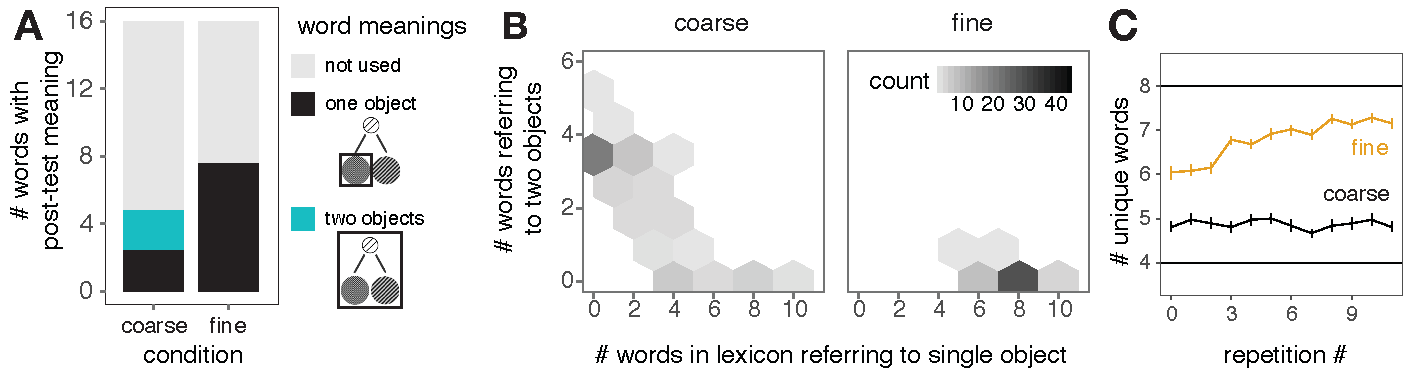
\includegraphics[scale=0.87]{sec2-results.pdf}
\caption{\emph{Comparison of simulation results to empirical data}. (A) Agents in our simulation learn to coordinate on a successful communication system, but converge faster in the coarse condition than the fine condition.  (B) The number of unique words used by agents in each repetition block increased in the fine condition but stayed roughly constant in the coarse condition. (C-D) The same metrics computed on our empirical data, qualitatively matching the patterns observed in the simulations. Each point is the mean proportion of correct responses by listeners; curves are nonparametric fits.}
\label{fig:sec2Results}
\end{center}
\end{figure}

\begin{figure}[h]
\begin{center}
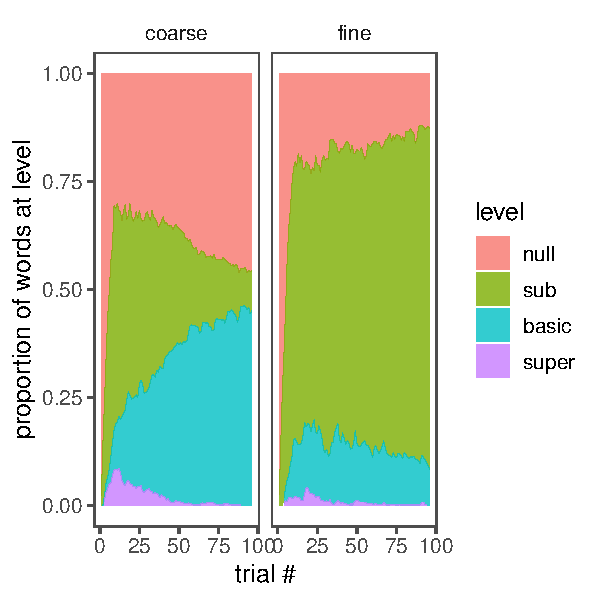
\includegraphics[scale=0.9]{evolution.pdf}
\caption{\emph{Dynamics of lexical beliefs over time in model simulations.} Regions represent the average proportion of words at each level of generality in an agent's beliefs about the lexicon. In the coarse condition, agents initially assume subordinate terms but gradually abstract away to a smaller number of more general terms; in the fine and mixed conditions, however, agents become more confident of subordinate terms.}
\label{fig:evolution}
\end{center}
\end{figure}

\subsubsection{Partners successfully learn to communicate}

First, we compare the model's learning curves across context conditions (Fig.~\ref{fig:sec2Results}A). 
We focus on the \emph{coarse} and \emph{fine} conditions for simplicity, since this single comparison captures the core phenomena of interest.
In a mixed-effects logistic regression, we find that communicative accuracy steadily improves over time across all conditions, $b=0.72, z = 16.9, p<0.001$.
However, accuracy also differed across conditions: adding a main effect of condition significantly improves model fit, $\chi^2(2) = 9.6, p = 0.008$. 
Accuracy is significantly higher in the coarse condition than the fine condition $b=-0.71, z=9.3, p <0.001$ and marginally higher than the mixed condition.

\subsubsection{Lexical conventions are shaped by context}

As an initial marker of context sensitivity, we examine the effective vocabulary sizes used by speakers in each condition.
We operationalized this measure by counting the total number of unique words produced within each repetition block.
This measure takes a value of 8 when a different word is consistently used for every object, and a value of 1 when exactly the same word is used for every object.
In an mixed-effects regression model including intercepts and random effects of trial number for each simulated trajectory, we find an overall main effect of condition, with agents in the fine condition using significantly more words across all repetition blocks ($m = 4.7$ in \emph{coarse}, $m=6.5$ in \emph{fine,} $t = 4.5, p < 0.001$).
However, we also found a significant interaction: the effective vocabulary size gradually increased over time in the fine condition, while it stayed roughly constant in in the coarse condition, $b = 0.18, t = 8.1, p < 0.001$, see Fig.~\ref{fig:sec2Results}B.

Next, we examine more closely the emergence of terms at different levels of generality.
We have access not only to the signaling behavior of our simulated agents, but also their internal \emph{beliefs} about their partner's lexicon, which allows us to directly examine the evolution of these beliefs from the beginning of the interaction.
At each time point in each game, we take the single meaning with highest probability for each word.
In Fig.~\ref{fig:evolution}, we show the proportion of words with meanings at each level of generality, collapsing across all games in each condition.


Qualitatively, we observe that agents begin by assuming null meanings (i.e. with an effectively empty vocabulary) but quickly begin assigning meanings to words based on their partner's usage.
In both conditions, basic-level meanings and subordinate-meanings are equally consistent with the initial data, but the simplicity prior prefers smaller effective vocabulary sizes where each word has smaller extensions.
After the first repetition block, however, agents in the coarse condition begin pruning out some of the subordinate-level terms and become increasingly confident of basic-level meanings.
Agents in the fine condition become even more confident of subordinate level meanings.

By the final trial, the proportion of basic-level vs.~subordinate-level terms is significantly different across the coarse and fine conditions.
Only 9\% of words had subordinate-level meanings (green) in the coarse condition, compared with 79\% in the fine condition, $\chi^2(1) = 436, p < 0.001$.
At the same time, 45\% of words had basic-level meanings (blue) in the coarse condition, compared with only 8\% in the fine condition, $\chi^2(1) = 136, p < 0.001$.
The remaining words in each condition were assigned the `null` meaning (red), consistent with an overall smaller effective vocabulary size in the coarse condition.
The diverging conventions across contexts are driven by Gricean expectations: because the speaker is assumed to be informative, only lexicons distinguishing between subordinate level objects can explain the speaker's behavior in the \emph{fine} condition.

\subsection{Experimental methods}

In this section, we evaluate our model's qualitative predictions about the effect of context on convention formation using an interactive behavioral experiment closely matched to our simulations.
We use a between-subjects design where pairs of participants are assigned to different communicative contexts and test the extent to which they converge on meaningfully different conventions.

\subsubsection{Participants}

We recruited 278 participants from Amazon Mechanical Turk to play an interactive, multi-player game.\footnote{This experiment was pre-registered at \url{https://osf.io/2hkjc/}. All statistical tests in mixed-effects models reported in this section use degrees of freedom based on the Satterthwaite approximation \cite{luke2017evaluating}.}.

\subsubsection{Procedure \& Stimuli}
Participants were paired over the web and placed in a shared environment containing an array of objects (Fig.~\ref{fig:context_design}A) and a `chatbox' to choose utterances from a fixed vocabulary by clicking-and-dragging (Fig.~\ref{fig:context_design}B). On each trial, one player (the `speaker') was privately shown a highlighted target object and allowed to send a single word to communicate the identity of this object to their partner (the `listener'), who subsequently made a selection from the array. Players were given full feedback, swapped roles each trial, and both received bonus payment for each correct response.

%The objects that served as referents were designed to cluster in a fixed three-level hierarchy with shape at the top-most level, color/texture at the intermediate levels, and frequency/intensity at the finest levels (see Fig.\ \ref{fig:context_design}C). Each communicative context contained four objects. Distractors could differ from the target at various level of the hierarchy, creating different types of contexts defined by the finest distinction that had to be drawn. 
%On \emph{fine} trials, the closest distractor belonged to the same fine-grained subordinate category (e.g.\ another striped circle; see Fig.\ \ref{fig:context_design}A).
%On \emph{coarse} trials, the closest distractor belonged to a coarser level of the conceptual hierarchy (e.g.\ dotted circle instead of striped circle).\footnote{Even coarser trials with super-ordinate distractors (e.g.\ a circle target among three square distractors) were logically possible but would have introduced several experimental confounds; we opted to leave these trial types out of our design and conduct the minimal manipulation.} 
We randomly generated distinct arrays of 16 utterances for each pair of participants (more than our model, which was restricted by computational complexity).
These utterances were created by stringing together consonant-vowel pairs into pronounceable 2-syllable words to reduce the cognitive load of remembering previous labels (see Fig.~\ref{fig:context_design}B)
These arrays were held constant across trials.

%Critically, we manipulated the statistics of the context in a between-subjects design to test the context-sensitivity of conventions. 
%In the \emph{fine} condition, all targets appeared in fine contexts; in the \emph{coarse} condition, all targets appeared in coarse contexts.
To match our model as closely as possible, pairs were assigned one of the same sequences of trials that we constructed for our simulations. 
In addition to behavioral responses collected over the course of the game, we designed a post-test to explicitly probe players' final lexica. For all sixteen words, we asked players to select all objects that a word can refer to (if any), and for each object, we asked players to select all words that can refer to it (if any). 
This bidirectional measure allowed us to check the internal validity of the lexica reported.
Pairs were randomly assigned to one of three different conditions, yielding $n=36$ dyads in the \emph{coarse} condition, $n=38$ in the \emph{fine} condition, and $n=53$ in the \emph{mixed} condition after excluding participants who disconnected before completion.

%\begin{figure}[t]
%\begin{center}
%{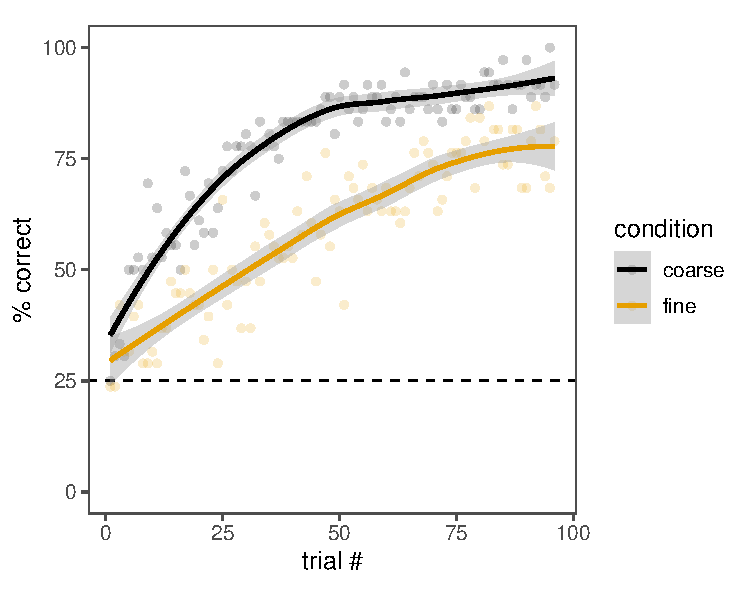
\includegraphics[scale=1]{./figures/sec2_empirical_accuracy.pdf}}
%{\caption{{
%\label{fig:context_accuracy}}}}
%\vspace{-3ex}
%\end{center}
%\end{figure}

\begin{figure}[t]
\begin{center}
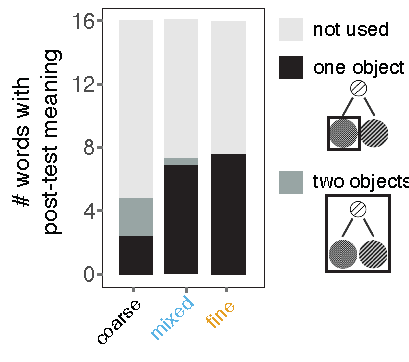
\includegraphics[scale=1]{./figures/Exp2_postTest}
\caption{\emph{Different lexicons emerge in different contexts.} Mean number of words, out of a word bank of 16 words, that human participants reported giving more specific meanings (black; applying to 1 object) or less specific meanings (dark grey; applying to 2 objects) in the post-test.}
\label{fig:sec2postTest}
\end{center}
\end{figure}


\subsection{Behavioral results}

\subsubsection{Partners successfully learn to communicate}

Although participants in all conditions began with no common basis for label meanings, performing near chance on the first trial (proportion correct $= 0.19$, 95\%~CI~$=~[0.13, 0.27]$), most pairs were nonetheless able to coordinate on a successful communication system over repeated interaction (see Fig.\ \ref{fig:sec2Results}C). 
A mixed-effects logistic regression on listener responses with trial number as a fixed effect, and including by-pair random slopes and intercepts, showed a significant improvement in accuracy overall, $z = 14.4, p < 0.001$. 
Accuracy also differed significantly \emph{across} conditions: adding an additional main effect of condition to our logistic model provided a significantly better fit, $\chi^2(2) = 10.8, p = 0.004$. 
Qualitatively, the \emph{coarse} condition was easiest for participants, the \emph{fine} condition was hardest, and the \emph{mixed} condition was in between.
These effects track the most important qualitative feature of our simulations -- our artificial agents were also able to successfully coordinate in both conditions, and did so more easily in the coarse condition than the fine condition. 
However, we found that the speed of coordination in the mixed and fine conditions was larger than predicted in our simulations.
The additional difficulty participants' experienced in the \emph{fine} condition may be due to additional motivational constraints, memory constraints, or other factors not captured in our model.


%Finally, the (log) response time taken by the speaker to choose an utterance also decreased significantly over the course of the game, $t(126) = -19.7, p < 0.001$, from approximately 20 seconds to only 6 seconds on average, indicating that lexical mappings became increasingly established or accessible.

%
%\paragraph{Partners converge on similar conventions}
%
%Another indicator of successful learning is convergence or alignment of lexica between partners within a dyad. 
%Using these estimates of each participant's lexicon, we compute the overlap between partners. 
%For most pairs, partners aligned strongly by the end, with a median post-test overlap of 97.6\% (125 out of 128 entries). 
%Because these matrices were extremely sparse, however, just a a few mismatches could have a large impact on performance. 
%Overall accuracy in the game is strongly correlated with alignment: partners who reported more similar lexica at the end also tended to perform significantly better at the task ($r = 0.77, t(120) = -13.5,~p <0.001$).  
%Despite these broad markers of convergence at the group level, individual performance had a long tail: a subpopulation of 29 games (11\% of coarse games, 18\% of mixed games, and 39\% of fine games) still showed relatively poor performance late in the game (see Fig.~\ref{fig:full_accuracy_grid} in Appendix for full histograms).
%For the subsequent analyses focusing on the content of the lexicon, we exclude games with accuracy below the pre-registered criterion of 75\% on the final quarter of trials to ensure we are examining only the content of lexica that converged.
%\rdh{double-check this. add better motivation if I do this.}

\subsubsection{Validating post-test responses}

Before examining post-test responses, we validate their internal consistency.
For each participant, we counted the number of mismatches between the two directions of the lexicon question (e.g.\ if they clicked the word `mawa' when we showed them one of the blue squares, but failed to click that same blue square when we showed `mawa'). 
In general, participants were highly consistent: out of 128 cells in the lexicon matrix (16 words $\times$ 8 objects), the median number of mismatches was 2 (98\% agreement), though the distribution has a long tail (mean $= 7.3$). 
We therefore conservatively take a participant's final lexicon to be the \emph{intersection} of their word-to-object and object-to-word responses for the subsequent analyses.

\subsubsection{Contextual pressures shape the lexicon}

We predicted that in contexts regularly requiring speakers to make fine distinctions among objects at subordinate levels of the hierarchy, we would find lexicalization of specific terms for each object (indeed, a one-to-one mapping may be the most obvious solution in a task with only 8 objects). 
Conversely, when no such distinctions were required, we expected participants to adaptively conventionalize more general terms that could be reused across different contexts.
One coarse signature of this prediction lies in the \emph{compression} of the resulting lexicon: less specific conventions should allow participants to achieve the same communicate accuracy with a smaller vocabulary.
To test this prediction, we operationalize vocabulary size as the number of words in each participant's reported lexicon in the post-test (i.e.\ the words for which they marked at least one object in the post-test in an internally consistent way). 
We then conducted a mixed-effects regression predicting each individual's vocabulary size as a function of dummy-coded condition factors, with random intercepts for each game. 
We found that participants in the \emph{coarse} condition reported significantly smaller, simpler lexica ($m = 4.9$ words) than participants in the \emph{mixed} ($m=7.1, t(110.8)=7.6, p < 0.001$) and \emph{fine} condition ($m = 6.9, t(109.3) = 6.4, p < 0.001$; see Fig.~\ref{fig:sec2postTest}). 

What allowed participants in the \emph{coarse} condition get away with fewer words in their lexicon while maintaining high accuracy?
We hypothesized that each word had a larger extension size. 
To test this hypothesis, we counted the numbers of `specific' terms (e.g.~words that refer to only one object) and more `general' terms (e.g.~words that refer to two objects) in the post-test. 
We found that the likelihood of lexicalizing more general terms differed systematically across conditions.
Participants in the \emph{coarse} condition reported significantly more general terms ($m=2.3$) than in the \emph{fine} ($m = 0.24, t(121.2) = 8.5, p < 0.001$) or \emph{mixed} ($m=0.65, t(122.7)= 7.3, p < 0.001$) conditions, where lexicons contained almost exclusively specific terms.
Using the raw extension size of each word as the dependent variable instead of counts yielded similar results.
Indeed, the modal system in the fine condition was exactly eight specific terms with no more general terms, and the modal system in the coarse condition was exactly four general terms (red, blue, striped, spotted) with no specific terms.
However, many individual participants reported a mixture of terms at different levels of generality (see Appendix Fig.~\ref{fig:mixtureOfTerms}). 

Finally, how did these lexica emerge over the course of interaction? 
We use the same measure of unique words produced in each repetition block that we used in our simulations (Fig.~\ref{fig:sec2Results}D). 
We constructed a mixed-effects regression model predicting the effective vocabulary size, including fixed effects of condition and repetition block, and random intercepts and effects of repetition block for each dyad. 
As in the post-test reports, we found an overall main effect of condition, with participants in the coarse condition using significantly fewer words across all repetition blocks: $m = 4.9$ in coarse, compared to $m=5.8, t(124)=6.1, p <0.001$ in mixed and $m=6.8, t(124) =11.4, p < 0.001$ in fine.
\textbf{[you've already given these stats above]}
Critically, however, we also found a significant interaction between block and condition. 
The effective vocabulary size gradually increased over time in the fine condition but remained roughly constant in the coarse condition, $b = 0.12, t = 4.5, p < 0.001$, see Fig.~\ref{fig:sec2Results}D.
This interaction, where participants initially attempt to reuse the same terms across targets in the fine condition, is consistent with a gradual differentiation based on communicative need.

%\paragraph{Model comparison}

%\rdh{TODO: we need to decide which comparisons are most interesting. may need to implement baseline model from other papers (e.g. Steels-style, or Spike et al. implementation?) for a more explicit comparison to models outside our class of Bayesian agents...}

%We compare our model to (1) a simpler case when both agents condition on the same data (i.e. the true target) even after an unsuccessful communication attempt, and (2) ask what happens when we manipulate forgetting parameter, or remove it?
%
%In a non-pragmatic variant of our model, agents use words proportional to their literal meaning and assume their partner is doing the same. 
%In this case, their lexicon converges to a degenerate 1-word (shape) state.
%Because an initial usage is consistent with all levels of abstraction, one of the agents will eventually extend the same word to different object. 
%Then the only way to subsequently accommodate this extension in the interaction history is to rule out more specific meanings. 
%The non-pragmatic agent has no way of knowing that this degenerate solution is confusing to their partner, and will continue to prefer it because it's literally true of every object.

\subsection{Discussion}

There is abundant evidence that languages adapt to the needs of their users.
Our model provides a cognitive account of how people coordinate on \emph{ad hoc} linguistic conventions that suit their immediate needs.
In this section, we evaluated predictions about context-sensitivity using new data from a real-time communication task.
When combined with the generalization mechanisms explored in the previous section, such rapid learning within dyadic interactions may be a powerful contributor allowing languages to adapt at the population-level over longer time scales.

Previous studies of convention formation have addressed context-sensitivity in different ways.
In some common settings, there is no explicit representation of context at all, as in the task known as the ``Naming Game'' where agents coordinate on names for objects in isolation \cite{steels2012experiments,baronchelli2008depth}. 
In other settings, communication is situated in a referential context, but this context is held constant, as in Lewis signaling games \cite{lewis_convention:_1969} where agents must distinguish between a fixed set of world states \cite{skyrms2010signals,BrunerEtAl14_LewisConventions}.
Finally, in the Discrimination Game \cite{steels2005coordinating,baronchelli2010modeling}, contexts are randomly generated on each trial, but have not been manipulated to assess context-sensitivity of the convention formation process.

%, which examined the joint formation of color categories and color naming conventions.
%As in our experiments, contexts were generated randomly on each trial from a large space and stimuli are embedded in a similarity space (with similarity based on Euclidean distance in continuous space rather than taxonomic relations).
%Unlike our task, contexts were not systematically manipulated, and the resulting level of generality was not evaluated: the only restriction was to ensure that color chips were a fixed minimum distance apart  \cite<see also>[which found that imposing a realistic Just Noticeable Difference function as the minimum distance on communicative contexts leads to human-like color naming systems]{baronchelli2010modeling}. \ks{not clear what point you were making in this paragraph}
%
In other words, context-sensitivity has typically been implicit in existing models. 
Models using simple update rules have accounted for referential context with a \emph{lateral inhibition} heuristic used by both the speaker and listener agents \cite{franke2012bidirectional,steels2005coordinating}.
If communication is successful, the connection strength between the label and object is not only increased, the connection between the label and competing objects (and, similarly, between the object and competing labels) is explicitly \emph{decreased} by a corresponding amount.
This lateral inhibition heuristic is functionally similar to our pragmatic reasoning mechanism, in terms of allowing the agent to learn from negative evidence (i.e. the speaker's choice \emph{not} to use a word, or the listener's choice \emph{not} to pick an object). 
%adele{let's talk more about this at some point: i used to argue the same that this type of statistical preemption was Gricean, but dogs do it too, so am less sure there's not a more mechanistic explanation}
Under our inferential framework, however, this property emerges as a natural consequence of well-established Gricean principles of pragmatic reasoning rather than as a heuristic.
%Reasoning about a partner's intentions, either while updating beliefs about their lexicon or while selecting an action, naturally instantiates a kind of inductive bias for \emph{mutual exclusivity} \cite{}.

%Our results may help to illuminate the relationship between our concepts and words, which are often treated interchangeably. While our mental taxonomies are adaptive to the natural perceptual structure of the world \cite{MervisRosch81_CategorizationReview} %(Rosch et al, 1976; Mervis \& Rosch ,1981; Murphy \& Smith, 1982), 
%it is far from inevitable that all levels of these conceptual hierarchies become conventionalized as lexical items. There are many perfectly natural concepts that are not represented by distinct words in the English language: for instance, we do not have words for each tree in our yards, or for ad-hoc concepts %like \emph{things to sell at a garage sale} 
%\cite{Barsalou83_AdHocCategories}. Indeed, English speakers are often fascinated by foreign words like the Danish ``hygge'' (a specific notion of coziness) or Scottish ``tartle'' (hesitating when introducing someone because you've forgotten their name) that are difficult to express in English.
%Our results highlight communicative needs to distinguish, in context, as a force behind the choice to lexicalize some fine-grained concepts. 
%A related direction for future work is to explore the relationship between communicative need and \emph{basic-level} structure.
%
%While we showed how abstract words emerge from efficiency even in a task requiring only reference to individual objects, there are other clear functional advantages to having abstract terms in the lexicon. For one, they allow speakers to efficiently refer to large, potentially infinite, sets of things, and make generalizations about categories, e.g.\ ``Dogs bark'' \cite{TesslerGoodman16_Generics}. Future work should explore this as an additional pressure toward abstract, nested nouns.
%Similarly, the option to refer to more specific concepts with compound terms (e.g.~``spotted dog''), which was not available in our experiment, may impact final conventions.
%We expect that labels will become lexicalized when the cost incurred by frequently using a compositional construction exceeds the cost of adding an additional word to the lexicon. 
%Future work should also explore these hypotheses about how lexicalization of nominal terms trades off with compositionality. 
%Our shared lexical conventions are richly structured systems with meanings at multiple levels of abstraction. 
%We are constantly supplementing our existing language with local conventions, as we need them.
